\documentclass[a4paper,12pt]{article}

%%% Работа с русским языком % для pdfLatex
\usepackage{cmap}					% поиск в~PDF
\usepackage{mathtext} 				% русские буквы в~фомулах
\usepackage[T2A]{fontenc}			% кодировка
\usepackage[utf8]{inputenc}			% кодировка исходного текста
\usepackage[english,russian]{babel}	% локализация и переносы
\usepackage{indentfirst} 			% отступ 1 абзаца
\usepackage{gensymb}				% мат символы?

%%% Работа с русским языком % для XeLatex
%\usepackage[english,russian]{babel}   %% загружает пакет многоязыковой вёрстки
%\usepackage{fontspec}      %% подготавливает загрузку шрифтов Open Type, True Type и др.
%\defaultfontfeatures{Ligatures={TeX},Renderer=Basic}  %% свойства шрифтов по умолчанию
%\setmainfont[Ligatures={TeX,Historic}]{Times New Roman} %% задаёт основной шрифт документа
%\setsansfont{Comic Sans MS}                    %% задаёт шрифт без засечек
%\setmonofont{Courier New}
%\usepackage{indentfirst}
%\frenchspacing

%%% Дополнительная работа с математикой
\usepackage{amsfonts,amssymb,amsthm,mathtools}
\usepackage{amsmath}
\usepackage{icomma} % "Умная" запятая: $0,2$ --- число, $0, 2$ --- перечисление
\usepackage{upgreek}

%% Номера формул
%\mathtoolsset{showonlyrefs=true} % Показывать номера только у тех формул, на которые есть \eqref{} в~тексте.

%%% Страница
\usepackage{extsizes} % Возможность сделать 14-й шрифт

%% Шрифты
\usepackage{euscript}	 % Шрифт Евклид
\usepackage{mathrsfs} % Красивый матшрифт

%% Свои команды
\DeclareMathOperator{\sgn}{\mathop{sgn}} % создание новой конанды \sgn (типо как \sin)
\DeclareMathOperator{\rg}{\mathop{rg}}
\DeclareMathOperator{\Rg}{\mathop{Rg}}
\DeclareMathOperator{\im}{\mathop{Im}}
\DeclareMathOperator{\tr}{\mathop{tr}}
\DeclareMathOperator{\const}{\mathop{const}}
\DeclareMathOperator{\Id}{\mathop{Id}}
%\DeclareMathOperator{\dim}{\mathop{dim}}
\usepackage{csquotes} % ещё одна штука для цитат
\newcommand{\pd}[2]{\ensuremath{\cfrac{\partial #1}{\partial #2}}} % частная производная
\newcommand{\abs}[1]{\ensuremath{\left|#1\right|}} % модуль
\renewcommand{\phi}{\ensuremath{\varphi}} % греческая фи
\newcommand{\pogk}[1]{\!\left(\cfrac{\sigma_{#1}}{#1}\right)^{\!\!\!2}\!} % для погрешностей


%\renewcommand{\labelenumi}{\asbuk{enumi})}

% Ссылки
\usepackage{color} % подключить пакет color
% выбрать цвета
\definecolor{BlueGreen}{RGB}{49,152,255}
\definecolor{Violet}{RGB}{120,80,120}
% назначить цвета при подключении hyperref
\usepackage[unicode, colorlinks, urlcolor=blue, linkcolor=blue, pagecolor=blue, citecolor=blue]{hyperref} %синие ссылки
%\usepackage[unicode, colorlinks, urlcolor=black, linkcolor=black, pagecolor=black, citecolor=black]{hyperref} % для печати (отключить верхний!)


%% Перенос знаков в~формулах (по Львовскому)
\newcommand*{\hm}[1]{#1\nobreak\discretionary{}
	{\hbox{$\mathsurround=0pt #1$}}{}}

%%% Работа с картинками
\usepackage{graphicx}  % Для вставки рисунков
\graphicspath{{images/}{images2/}}  % папки с картинками
\setlength\fboxsep{3pt} % Отступ рамки \fbox{} от рисунка
\setlength\fboxrule{1pt} % Толщина линий рамки \fbox{}
\usepackage{wrapfig} % Обтекание рисунков и таблиц текстом
\usepackage{multicol}

%%% Работа с таблицами
\usepackage{array,tabularx,tabulary,booktabs} % Дополнительная работа с таблицами
\usepackage{longtable}  % Длинные таблицы
\usepackage{multirow} % Слияние строк в~таблице
\usepackage{caption}
\captionsetup{labelsep=period, labelfont=bf}

%%% Оформление
\usepackage{indentfirst} % Красная строка
%\setlength{\parskip}{0.3cm} % отступы между абзацами
%%% Название разделов
\usepackage{titlesec}
\titlelabel{\thetitle.\quad}
\renewcommand{\figurename}{\textbf{Рис.}}		%Чтобы вместо figure под рисунками писал "рис"
\renewcommand{\tablename}{\textbf{Таблица}}		%Чтобы вместо table над таблицами писал Таблица
\usepackage{enumitem}
\setlist{nolistsep}
\usepackage{verbatim}

%%% Теоремы
\theoremstyle{plain} % Это стиль по умолчанию, его можно не переопределять.
\newtheorem{theorem}{Теорема}[section]
\newtheorem{proposition}[theorem]{Утверждение}
\newtheorem{predlog}{Предложение}[section]
\newtheorem{lemma}{Лемма}[section]

\theoremstyle{definition} % "Определение"
\newtheorem{definition}{Определение}[section]
\newtheorem{corollary}{Следствие}[theorem]
\newtheorem{problem}{Задача}[section]

\theoremstyle{remark} % "Примечание"
\newtheorem*{nonum}{Решение}
\newtheorem{zamech}{Замечание}[theorem]

%%% Правильные мат. символы для русского языка
\renewcommand{\epsilon}{\ensuremath{\varepsilon}}
\renewcommand{\phi}{\ensuremath{\varphi}}
\renewcommand{\kappa}{\ensuremath{\varkappa}}
\renewcommand{\le}{\ensuremath{\leqslant}}
\renewcommand{\leq}{\ensuremath{\leqslant}}
\renewcommand{\ge}{\ensuremath{\geqslant}}
\renewcommand{\geq}{\ensuremath{\geqslant}}
\renewcommand{\emptyset}{\varnothing}

%%% Для лекций по инфе
\usepackage{alltt}
\newcounter{infa}[section]
\newcounter{num}
\definecolor{infa}{rgb}{0, 0.2, 0.89}
\definecolor{infa1}{rgb}{0, 0.3, 1}
\definecolor{grey}{rgb}{0.5, 0.5, 0.5}
\newcommand{\tab}{\ \ \ }
\newcommand{\com}[1]{{\color{grey}\##1}}
\newcommand{\num}{\addtocounter{num}{1}\arabic{num}\tab}
\newcommand{\defi}{{\color{infa}def}}
\newcommand{\ini}{{\color{infa}in}}
\newcommand{\rangei}{{\color{infa}range}}
\newcommand{\fori}{{\color{infa}for}}
\newcommand{\ifi}{{\color{infa}if}}
\newcommand{\elsei}{{\color{infa}else}}
\newcommand{\printi}{{\color{infa1}print}}
\newcommand{\maxi}{{\color{infa}max}}
\newcommand{\classi}{{\color{infa}class}}
\newcommand{\returni}{{\color{infa}return}}
\newcommand{\elifi}{{\color{infa}elif}}


\newenvironment{infa}[1]{
	
	\vspace{0.5cm}
	\addtocounter{infa}{1}%
	\noindent{\large \textbf{Программа №\thesection.\arabic{infa}}}\textbf{<<#1>>}%
	\begin{alltt}%
	}{\end{alltt}
	\setcounter{num}{0}
	\vspace{0.1cm}}
%Пример кода:
%\begin{infa}{Поразрядная сортировка}
%	\ \num \defi count_sort(a):\tab \com{определяет нашу функцию}
%	\ \num \tab m = \maxi(a)+1
%	\ \num \tab q = [0]*m
%	\ \num \tab \fori x \ini a:
%	\ \num \tab \tab q[x] += 1
%	\ \num \tab pos = 0
%	\ \num \tab \fori x \ini q:
%	\ \num \tab \tab \fori i \ini \rangei(q[x]):
%	\ \num \tab \tab \tab a[pos] = x
%	\num \tab \tab \tab pos += 1
%\end{infa}

\usepackage{titlesec}
\titlelabel{\thetitle.\quad}


\usepackage{graphicx,xcolor,adjustbox,setspace}

\newcommand{\resh}{\noindent\textit{Решение:}\\}

\newcounter{prim}
\newenvironment{prim}{%
	\addtocounter{prim}{1}
	\noindent{\\
		\textbf{\noindentПример \arabic{prim}\\}}%
}{\vspace{2mm}\\
	\resh
}
\definecolor{orange}{rgb}{1, 0.7, 0.1}
%\usepackage{ulem}

\usepackage{bm} %жирный греческий шрифт

\newenvironment{psm}
{\left(\begin{smallmatrix*}[r]}
	{\end{smallmatrix*}\right)}

\newenvironment{pmatrixr}
{\begin{pmatrix*}[r]}
	{\end{pmatrix*}}

\renewcommand{\figurename}{\textbf{Рис.}}		%Чтобы вместо figure под рисунками писал "рис"
\renewcommand{\tablename}{\textbf{Таблица}}		%Чтобы вместо table над таблицами писал Таблица


\title{3.3.2}
\author{Кутушева Алиса}
\date{today}
\usepackage[left=1.27cm,right=1.27cm,top=1.27cm,bottom=2cm]{geometry}
\begin{document}
	
	\begin{titlepage}
		\begin{center} 
			
			\large Московский физико-технический институт\\
			Факультет молекулярной и химической физики\\
			\vspace{7cm}
			\huge Лабораторная работа № 3.2.4\\
			\textbf{\Large <<Свободные колебания в электрическом контуре>>}\\
		\end{center} 
		
		\vspace{7.5cm}
		{\par \raggedleft \large \emph{Выполнили:}\\ студенты 2 курса\\ 641 группы ФМХФ\\ Кутушева Алиса\\ Ильдаровна \\ \& \\Горшков Тимофей \\Владимирович \par}
		\begin{center}
			\vfill Москва 2017
		\end{center}
	\end{titlepage}
\newpage
\setcounter{page}{2}

\begin{center}
	\vspace*{-0.5cm}{
		\textbf{Аннотация:}\\ 
		\vspace{0.2cm}
		\parbox{16cm}{ 
			\tab В~этом отчёте изложены результаты выполнения лабораторной работы <<Свободные колебания в электрическом контуре>>. В данной работе исследуются зависимость периода свободных колебаний контура от ёмкости, зависимость логарифмического декремента затухания от сопротивления. По резултатам измерений определяетя критическое сопротивление и добротность контура.
		}
	}
\end{center}

	\hspace{0.2cm}\textbf{Цель работы:}
	\par исследование свободных колебаний в колебательном контуре.


	\hspace{0.2cm}\textbf{В работе используются:}
	\par генератор импульсов Г5-54, электронное реле, магазин сопротивлений P33, магазин ёмкостей P5025, индуктивность, электронный осциллограф, универсальный мост GWINSTEK LCR-7819.
	
\section{Теоретические сведения}
\par Исследуемый колебательный контур состоит из индуктивности $L$, ёмкости $С$ и резистора $R$ (рис. 1). Конденсатор контура заряжается короткими одиночными импульсами, после каждого из которых в контуре возникают свободные затухающие колебания. Уравнение колебаний:
\begin{equation}
{\ddot{I} + 2 \gamma \dot{I} + {w_0}^2 I = 0}
\end{equation}




\par Подав напряжение с конденсатора на осциллограф, можно по картине, возникающей на экране осциллографа, определить период колебаний в контуре, исследовать затухание колебаний и определить основные параметры колебательного контура.

\begin{wrapfigure}{r}{0.4\textwidth}
	\fbox{
		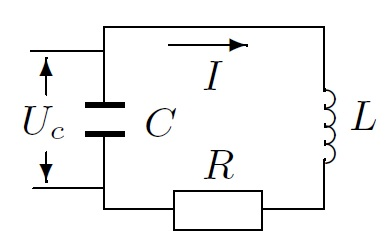
\includegraphics[width=\linewidth]{S_K1}}
	\caption{Колебательный контур.}
	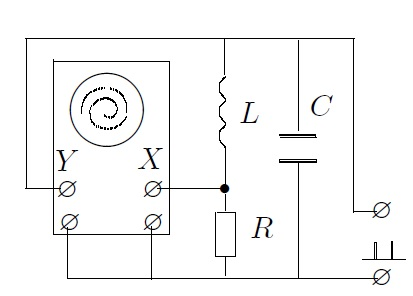
\includegraphics[width=\linewidth]{S_K2}
	\caption{Схема установки для наблюдения затухающих колебаний на фазовой плоскости.}
	\label{mah}
	\vspace{-2cm}
\end{wrapfigure}

\par Картину колебаний можно представить не только в координатах $(U, t)$, но и в координатах $(U, \dot{U})$, или, как говорят, на фазовой плоскости. В этих координатах кривая незатухающих колебаний ($\gamma $ = 0) имеет вид эллипса (или окружности — при одинаковых амплитудах $U$ и $\dot{U}$, а картина реальных колебаний изображается сворачивающейся спиралью. 
\begin{comment}
\begin{wrapfigure}{r}{\linewidth}
		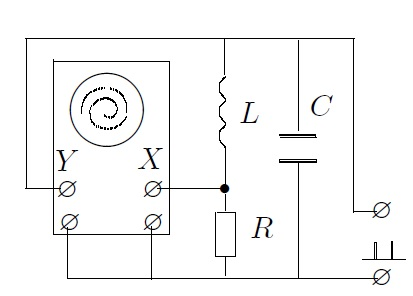
\includegraphics[width=0.5\linewidth]{S_K2}
	\caption{Схема}%Схема установки для наблюдения затухающих колебаний на фазовой плоскости.
	\label{mah}
	%\vspace{-3cm}
\end{wrapfigure}
\end{comment}
\par Схема подключения осциллографа для изучения колебаний на фазовой плоскости представлена на рис. 2. На вертикальный вход осциллографа подаётся напряжение $U_c$ с конденсатора, а на горизонтальный — напряжение с резистора. $U_R (U_R \sim I \sim dq/dt \sim dU_c/dt) $


\section{Экспериментальная установка}

\par На рис. 3 приведена схема для исследования свободных колебаний в контуре, содержащем постоянную индуктивность $L$ и переменные ёмкость $С$ и сопротивление $R$.
Колебания наблюдаются на экране осциллографа.

\par Для периодического возбуждения колебаний в контуре используется генератор импульсов Г5-54. С выхода генератора по коаксиальному кабелю импульсы поступают на колебательный контур через электронное реле, смонтированное в отдельном блоке (или на выходе генератора). Реле содержит диодный тиристор $D$ и ограничительный резистор $R_1$.

\par Импульсы заряжают конденсатор $С$. После каждого импульса генератор отключается от колебательного контура, и в контуре возникают свободные затухающие колебания. Входное сопротивление осциллографа велико ($\sim$1 МОм), так что его влиянием на контур можно пренебречь. Для получения устойчивой картины затухающих колебаний используется режим ждущей развёртки с синхронизацией внешними импульсами, поступающими с выхода «синхроимпульсы» генератора.

\begin{comment}
\begin{figure}
	\centering
	\fbox{
		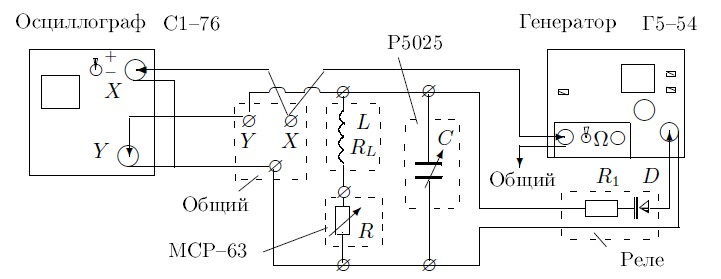
\includegraphics[width=\linewidth]{S_K3}}
	\caption{Схема установки для исследования свободных колебаний}
	\label{mah}
\end{figure}
\end{comment}
\section{Ход работы}

\par \textit{1)Измерение периодов}
\par 1. Установим на магазине сопротивлений величину $R = 0$; на магазине ёмкостей — величину $C = 0,02$ мкФ.
\par 2. Прокалибруем горизонтальную ось осциллографа по известному периоду повторения импульсов: для этого
\par а) подберём частоту развёртки осциллографа, при которой расстояние $x_0$ между импульсами, поступающими с генератора ($T_0 = 0,01$ с), занимает почти весь экран: $x_0 = 10$;
\par б) измерив на экране расстояние $x$, которое занимают несколько полных периодов $n$, рассчитаем период колебаний контура: $T = T_0 x/(n x_0)$. 
Изменяя ёмкость от 0,02 мкФ до 0,9 мкФ и периодически проверяя величину $x_0$, проведем измерения периодов (9 значений). Данные занесем в таблицу 1.

\begin{table}[h!!!]
	\centering
	\caption{ Измерение периодов }
	
	\begin{tabular}{|c|c|c|c|c|c|c|c|}
		\hline 
		№ & $C$, $ 10^{-2} $ мкФ & $x$ & $n$ & $T_e$, $10^{-4}$ c & $\Delta T_e$, $10^{-4}$ & $T_t$,$10^{-4}$&  $\Delta T_t$, $10^{-4}$\\ 
		\hline 
		1 & 2 & 0,8 & 2 & 4,0 & 1,1 & 4,0 & 0,5\\ 
		\hline 
		2 & 13 & 4,2 & 4 & 10,5 & 0,7 & 10,1 & 0,2\\ 
		\hline 
		3 & 24 & 4,2 & 3 & 14,0 & 0,9 & 13,80 & 0,15 \\ 
		\hline 
		4 & 35 & 8,4 & 5 & 16,8 & 0,7 & 16,67 & 0,12\\ 
		\hline 
		5 & 46 & 5,8 & 3 & 19 & 1 & 19,11 & 0,11 \\ 
		\hline 
		6 & 57 & 6,4 & 3 & 21,3 & 1,1 & 21,2 & 0,1 \\ 
		\hline 
		7 & 68 & 7 & 3 & 23,3 & 1,1 & 23,23 & 0,09\\ 
		\hline 
		8 & 79 & 7,6 & 3 & 25,3 & 1,2 & 25,03 & 0,09\\ 
		\hline 
		9 & 90 & 5,4 & 2 & 27,0 & 1,5 & 26,72 & 0,08\\ 
		\hline 
	\end{tabular} 
	
\end{table}

\par \textit{2)Критическое сопротивление и декремент затухания}
\par 1. Приняв $L = 200$ мГн, рассчитаем ёмкость $С$, при которой собственная частота колебаний контура $ \nu_0 = 1/(2\pi \sqrt{LC}) $ составляет 5 кГц : $C = \frac{1}{4\pi^2 \nu_0^2 L} = 5,1 \cdot 10^{-9}$ Ф. Для выбранных значений $L$ и $С$ рассчитаем критическое сопротивление контура $R_{kp}$ по формуле $R_{kp} = 2 \sqrt{L/C} = (1,250 \pm 0,003) \cdot 10^4$ Ом. Погрешность считаем по формуле: $\Delta R = \sqrt{\frac{(\Delta L)^2}{LC} + \frac{L (\Delta C)^2}{C^3}}$
\par 2. Установим на магазине ёмкость, близкую к рассчитанной. Увеличивая сопротивление $R$ от 0 до $R_{kp}$, проблюдаем картину затухающих колебаний на экране осциллографа. Зафиксируем сопротивление магазина, при котором колебательный режим переходит в апериодический: $R_{kp} = (0,997 \pm 0,002) \cdot 10^4$ Ом.
\par 3. Установим сопротивление $R \simeq 0,1 R_{kp}$ (эксп.). Получим на экране картину затухающих колебаний. Для расчёта логарифмического декремента затухания $\Theta$ по формуле $\Theta = \frac{1}{n} \ln \frac{U_k}{U_{k+n}}$ измерим амплитуды, разделённые целым числом периодов $n$. Повторим измерения для 7 значений $R$, лежащих в интервале ($0,1\div 0,3) \cdot R_{kp}$. Данные занесем в таблицу 2.
\begin{table} 
	\centering
	\caption{ Данные для декремента затухания }

\begin{tabular}{|c|c|c|c|c|c|} 
	\hline 
	$R$,кОм & $U_k$ & $n$ & $U_{k+n}$ & $\Theta$ & $\Delta \Theta$\\ 
	\hline 
	1 & 5,4 & 2 & 1,8 & 0,55 & 0,07\\ 
	\hline 
	1,3 & 5,4 & 2 & 1,3 & 0,7 & 0,1 \\ 
	\hline 
	1,5 & 5,4 & 1 & 2,4 & 0,81 & 0,12\\ 
	\hline 
	2 & 5,4 & 1 & 1,8 & 1,10 & 0,15\\ 
	\hline 
	2,3 & 5,4 & 1 & 1,6 & 1,22 & 0,16\\ 
	\hline 
	2,5 & 5,4 & 1 & 1,4 & 1,35 & 0,18\\ 
	\hline 
	3 & 5,4 & 1 & 1 & 1,7 & 0,2 \\ 
	\hline 
\end{tabular} 
\end{table}
	
\par \textit{3) Колебания на фазовой плоскости}
\par 1. Пронаблюдаем затухающие колебания на фазовой плоскости. При том же значении $C = 5,1 \cdot 10^{-9}$ Ф, наблюдаем за изменением спирали при увеличении сопротивления в интервале ($0,1\div 0,3) \cdot R_{kp}$.
Для определения $\Theta$ измерим радиусы витков спирали, разделённые целым числом периодов $n$, для двух значений $R$ на каждом краю рабочего диапазона. Данные занесем в таблицу 3.

\begin{table}[h!]
	\centering
	\caption{ Колебания на фазовой плоскости }
	
	\begin{tabular}{|c|c|c|c|c|c|}
		\hline 
		$R$,кОм & $U_k$ & $n$ & $U_{k+n}$ & $\Theta$ &  $\Delta \Theta$ \\ 
		\hline 
		1 & 0,6 & 2 & 1,8 & 0,6 & 0,2 \\ 
		\hline 
		1,3 & 0,8 & 1 & 1,6 & 0,7 & 0,4 \\ 
		\hline 
		2,7 & 0,8 & 1 & 3,7 & 1,5 & 0,3\\ 
		\hline 
		3 & 0,6 & 1 & 2,8 & 1,5 & 0,4\\ 
		\hline 
	\end{tabular} 
	
\end{table}

2. Измерим индуктивность $L$ и омическое сопротивление катушки $R_L$ с помощью моста переменного тока при разных частотах. Данные занесем в таблицу 4.

\begin{table} [h!]
	\centering
	\caption{ Частотная зависимость параметров установки }
	
	\begin{tabular}{|c|c|c|c|c|}
		\hline 
		$\nu$, Гц & 50 & 100 & 1000 & 5000 \\ 
		\hline 
		$R$,Ом & 11 & 11,3 & 18,8 & 46,8 \\ 
		\hline 
		$L$,мГн & 203 & 201 & 199 & 200 \\ 
		\hline 
	\end{tabular} 
	
\end{table}

\section{Обработка результатов}

\par 1. Рассчитаем теоретические значения периодов по формуле $T = 2\pi \sqrt{LC}$. Рассчитаем погрешности $\Delta T_t = \frac{\pi}{\sqrt{LC}}(C \cdot \Delta L + L \cdot \Delta C) $; $\Delta T_e = T_e (\frac{\Delta x}{x} + \frac{\Delta x_0}{x_0}) $. Данные занесем в таблицу 1. Построим график $T_{e}(T_{t})$.
\begin{figure}
	\centering
	\fbox{
		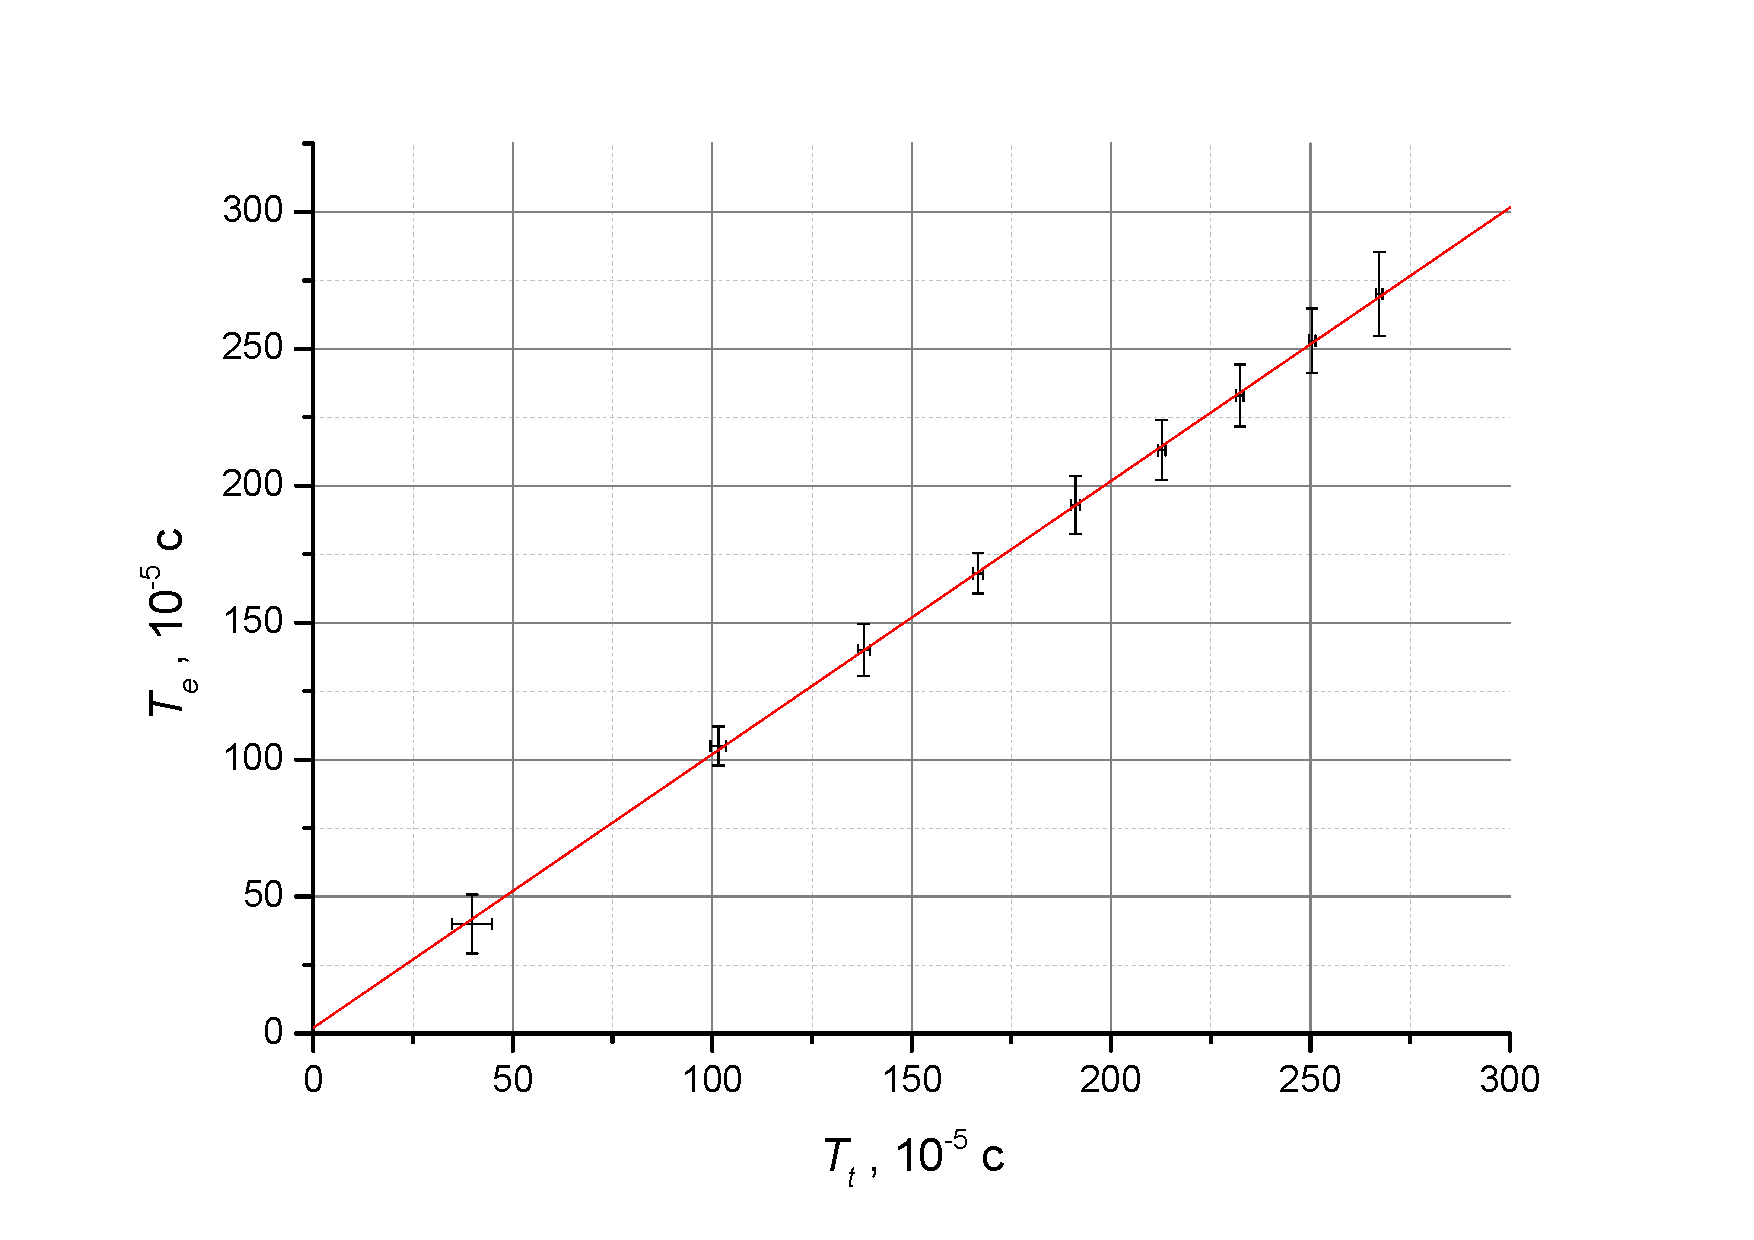
\includegraphics[width=\linewidth]{S_K4}}
	\caption{График зависимости экспериментального периода от теоритического}
	\label{mah}
\end{figure}

\par 2. Рассчитаем значения $\Theta$  и $R_k$ (сопротивление контура, состоит из сопротивления магазина $R$ и омического сопротивления катушки $R_L$). Рассчитаем погрешности $1/\Theta^2$ и $1/R^2_k$: 
\par $\Delta \Theta = \frac{1}{n} \cdot \Big(\frac{\Delta U_n}{U_n} + \frac{\Delta U_{n+k}}{U_{n+k}}), \Delta (1/\Theta^2) = \frac{2\Delta \Theta}{\Theta^3}$; $\Delta R_L = 5 \cdot 10^{-4} \cdot 11,3$ Ом  - мало по сравнению с $\Delta R_p = 0,002 \cdot R_d$, где $R_p$ - сопротивление моста, а $R_d$ - сопротивление текущей декады. Тогда погрешность $1/R^2 = 2 \cdot \Delta R_p / R^3$. Данные занесем в таблицу 5.

\begin{table} [h!]
	\centering
	\caption{ Данные для определения критического сопротивления }
	\begin{tabular}{|c|c|c|c|}
		\hline 
		$1/R^2$,1/Ом$^2$ & $\Delta (1/R^2)$,1/Ом$^2$ & $1/\Theta^2$ & $\Delta (1/\Theta^2)$ \\ 
		\hline 
		0,978 & 0,004 & 3,3 & 0,5 \\ 
		\hline 
		0,582 & 0,002 & 1,98 & 0,09 \\ 
		\hline 
		0,4378 & 0,0017 & 1,52 & 0,11 \\ 
		\hline 
		0,247 & 0,001 & 0,83 & 0,14 \\ 
		\hline 
		0,1872 & 0,0007 & 0,67 & 0,18 \\ 
		\hline 
		0,1586 & 0,0006 & 0,6 & 0,6 \\ 
		\hline 
		0,1103 & 0,0005 & 0,35 & 0,12 \\ 
		\hline 
	\end{tabular} 
	
\end{table}

\par Построим график в координатах $1/\Theta^2 = f(1/R^2_k)$. Определим критическое сопротивление $R_{kp}$ по наклону прямой. Приняв обозначения: $1/\Theta^2 = Y, 1/R^2_k = X$, получим: $R_{kp} = 2\pi \sqrt{\frac{\Delta Y}{\Delta X}} =  2\pi \sqrt{3,44 \cdot 10^6} = 11653$ Ом. Оценим погрешность: $\pi \Delta k / \sqrt{k} = 90$ Ом. Итого: $R_{kp} = (11650 \pm 90)$ Ом.

\begin{figure}
	\centering
	\fbox{
		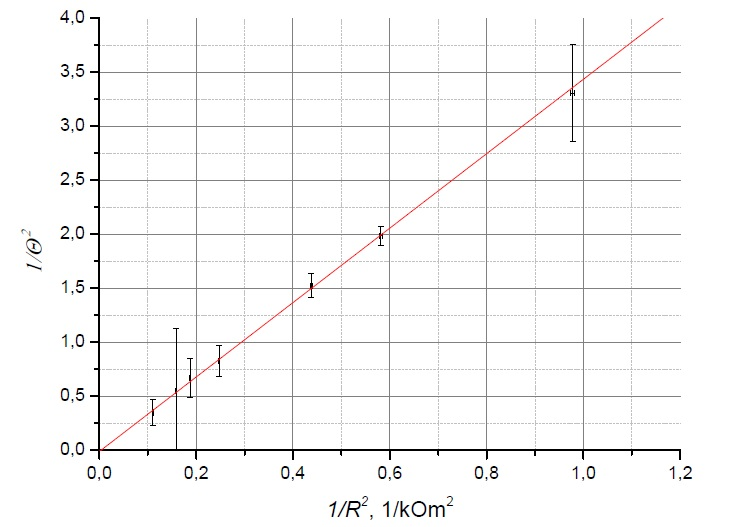
\includegraphics[width=\linewidth]{S_K5}}
	\caption{График для определения критического сопротивления, $\frac{\Delta Y}{\Delta X} = (3,44 \pm 0,05)\cdot 10^6$ Ом$^2$.}
	\label{mah}
\end{figure}

\par 3. Рассчитаем добротность контура для максимального и минимального значений $\Theta$, используя равенствo $Q = \frac{\pi}{\Theta}$. Рассчитаем погрешность $Q$: $\Delta Q = \frac{\pi \Delta \Theta}{\Theta^2}, \Delta \Theta = \frac{1}{n}(\frac{\Delta U_1}{U_1} + \frac{\Delta U_2}{U_2}) $ 
\par $\Theta_{min} = 0,55 \pm 0,07 \Rightarrow Q_{max} = 5,7 \pm 0,8; \Theta_{max} = 1,7 \pm 0,2 \Rightarrow Q_{min} = 1,86 \pm 0,3.$ 
\par Сравним $Q$ с расчетом через параметры $R,L$ и $C$: $Q = \frac{1}{R} \sqrt{\frac{L}{C}}.$ Рассчитаем погрешность $Q: \Delta Q = \sqrt{\frac{L \Delta R^2}{C R^4} + \frac{\Delta L^2}{4 R^2LC} + \frac{L \Delta C^2}{4 R^2C^3}}$
\par $Q_{max} = 6,278 \pm 0,014; Q_{min} = 2,093 \pm 0,005.$
\par 4. Рассчитаем величину $\Theta$ на фазовой плоскости по тем же соотношениям. $\Theta_{min} = 0,6 \pm 0,2;$ $ \Theta_{max} = 1,5 \pm 0,4$.

\section{Обсуждение результатов и выводы}
\par В ходе данной работы:
\par 1)Была получена зависимость $T_e(T_t)$ которая подтвердила справедливость соотношения $T = 2 \pi \sqrt{LC}$
\par 2) Тремя разными способами было получено значение $R_{kr}$: Теоретически $R = (12500 \pm 30) Ом$, графически $R = (11650 \pm 90) Ом$, экспериментально $R = (9970 \pm 20) Ом$. Все 3 значения разошлись.
\par 3) Были получены декременты затухания при измерении $R_{kp}$ и при наблюдении колебаний на фазовой плоскости: $\Theta_{min} = 0,55 \pm 0,07$ и $\Theta_{min} = 0,6 \pm 0,2; \Theta_{max} = 1,7 \pm 0,2$ и $\Theta_{max} = 1,5 \pm 0,4$.
\end{document}